Um die Implementierung eines 6LoWPAN-Netzwerks mit Contiki beispielhaft darzulegen, haben wir ein Netzwerk bestehend aus mehreren Nodes und einem Edge-Router selbst programmiert. Die Nodes können über eine \ac{uart} Schnittstelle mit dem Nutzer interagieren. Im realen Einsatz wäre zwar eine Machine-to-Machine-Kommunikation wünschenswert, jedoch würde diese zu einem weniger anschaulichen Ergebnis führen. \\
Um die einzelnen Nodes und gegebenenfalls den Edge-Router zu programmieren, haben wir eine kleine Skriptsprache bestehend aus wenigen Befehlen entwickelt. So kann beispielsweise die eigene IP-Adresse abgefragt werden oder es können Pakete mit dem gewünschten Inhalt an Empfänger innerhalb und außerhalb des Netzwerks geschickt werden. \\
Weil die Implementierung eines richtigen Edge-Routers wie er in 6LoWPAN definiert ist den Rahmen dieses Projekts sprengen würde, haben wir uns einer Hilfslösung bedient. Im 6LoWPAN fungiert ein Teilnehmer mit leicht verändertem Code als Ziel für Pakete, die das Netzwerk verlassen sollen. Diese Pakete sind auf der IP-Schicht und UDP-Schicht an eben diesen Teilnehmer adressiert und enthalten die Adressen bzw. den Ports des eigentlichen Empfängers in der Payload. Der Teilnehmer erkennt ein solches Paket und schickt die Nutzdaten, die Quell- und Zieladresse, und den Quell- sowie Zielport über UART an einen anderen Controller. Dieser wiederum generiert aus der UART-Nachricht ein UDP/IP-Paket und schickt es über Ethernet an den Adressaten.\\
Will ein Teilnehmer außerhalb des 6LoWPAN eine Node innerhalb dieses Netzwerks erreichen, so schickt er ein Paket, das auf UDP- und IP-Schicht an den UART-Partner des 6LoWPAN adressiert ist und Zieladresse und Port wiederum nebst eigentlichen Nutzdaten in der Payload enthält. Wieder werden die relevanten Daten über UART ausgetauscht und im 6LoWPAN an den richtigen Empfänger weitergeleitet. Mit wenigen Einschränkungen kann man also das über UART kommunizierende Bündnis in seiner Gesamtheit als Edge-Router betrachten. Abbildung \ref{beispielnetzwerk} zeigt den Aufbau des Projekts anschaulich.\\
\begin{figure}
	\centering
	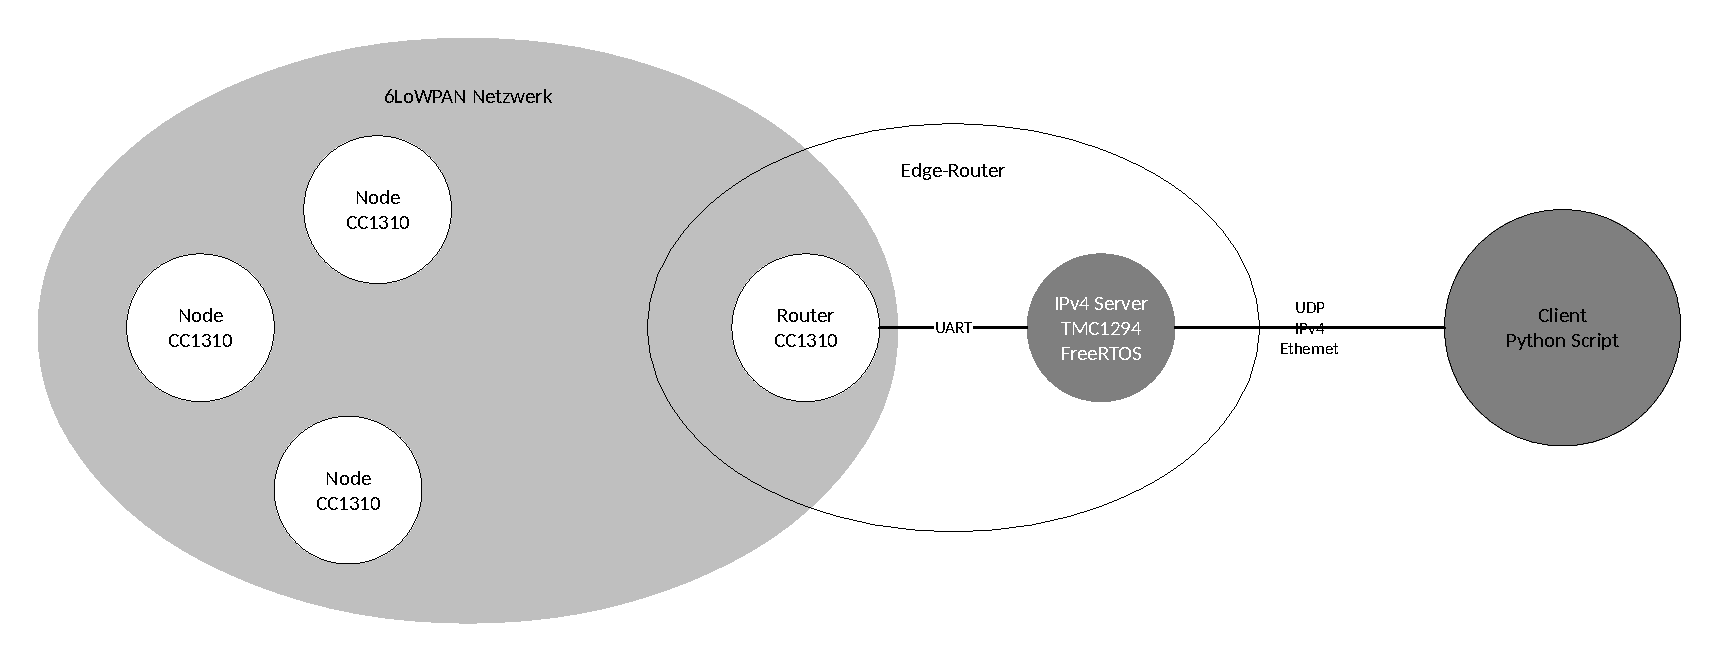
\includegraphics[width=\textwidth]{Grafiken-Alex/beispielnetzwerk.pdf}
	\caption{Der Aufbau unseres Beispielnetzwerks}
	\label{beispielnetzwerk}
\end{figure}

\subsection{Eingesetzte Hardware}
Die einzelnen Nodes bestehen hauptsächlich aus dem CC1310, einem 15.4-fähigen Mikrocontroller von Texas Instruments. Um die Arbeit mit diesem Controller zu vereinfachen, wurden das zugehörige Launchpad verwendet, welches vor allem durch die bereits bestehende Antenne den Entwicklungsaufwand stark reduziert und es uns ermöglichte, uns auf das eigentlich wesentliche Thema zu konzentrieren. \\
Auch der Edge-Router besteht 6LoWPAN-seitig aus einem CC1310 Launchpad. Dieses ist durch eine einfache Jumper-Verbindung, die die UART-Kommunikation ermöglicht mit einem TI129EXL-Launchpad verbunden. Dieses wiederum bietet die Möglichkeit der Kommunikation nach außen durch Ethernet. 

\subsection{Konventionen}
Um ein ordentliches Routing von Paketen durch den Edge-Router zu ermöglichen, mussten gewisse Konventionen ausgearbeitet werden. Diese beinhalten den Aufbau eines Pakets, dessen Source oder Destination außerhalb des 6LoWPAN liegt in der Kommunikation zwischen
\begin{itemize}
	\item Node und Edge-Router über IEEE 802.15.4
	\item CC1310 und TI1294 über UART
\end{itemize}
Es war nicht möglich, hier den gleichen Paketaufbau einzusetzen, weil über UART in den Nutzdaten, Informationen mitgeteilt werden, die über 15.4 schon durch die Header ersichtlich sind - beispielsweise die IPv6-Adresse des 6LoWPAN-seitigen Kommunikationspartners. Die Grafiken \ref{komm-intern} und \ref{komm-extern} zeigen den jeweiligen Aufbau eines Routing-Pakets.

\begin{figure}
	\centering
	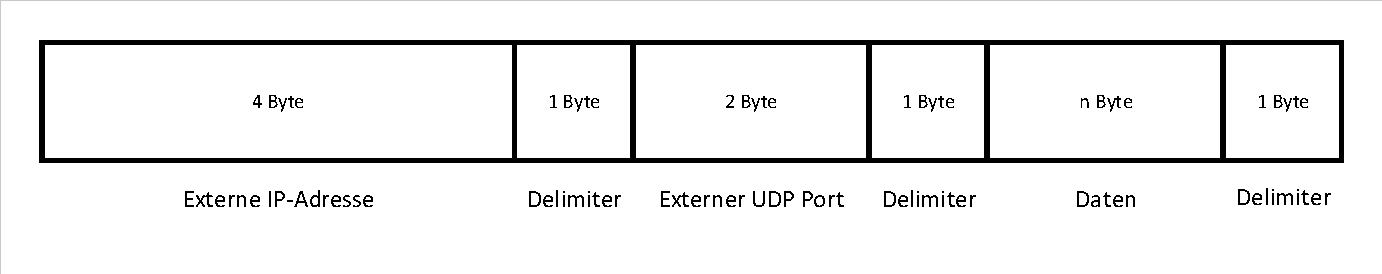
\includegraphics[width=\textwidth]{Grafiken-Alex/komm-intern.pdf}
	\caption{Aufbau eines Routing-Pakets innerhalb des 6LoWPAN. Als Delimiter wird 0x2E (entspricht in ASCII einem Punkt) eingesetzt.}
	\label{komm-intern}
\end{figure}
\begin{figure}
	\centering
	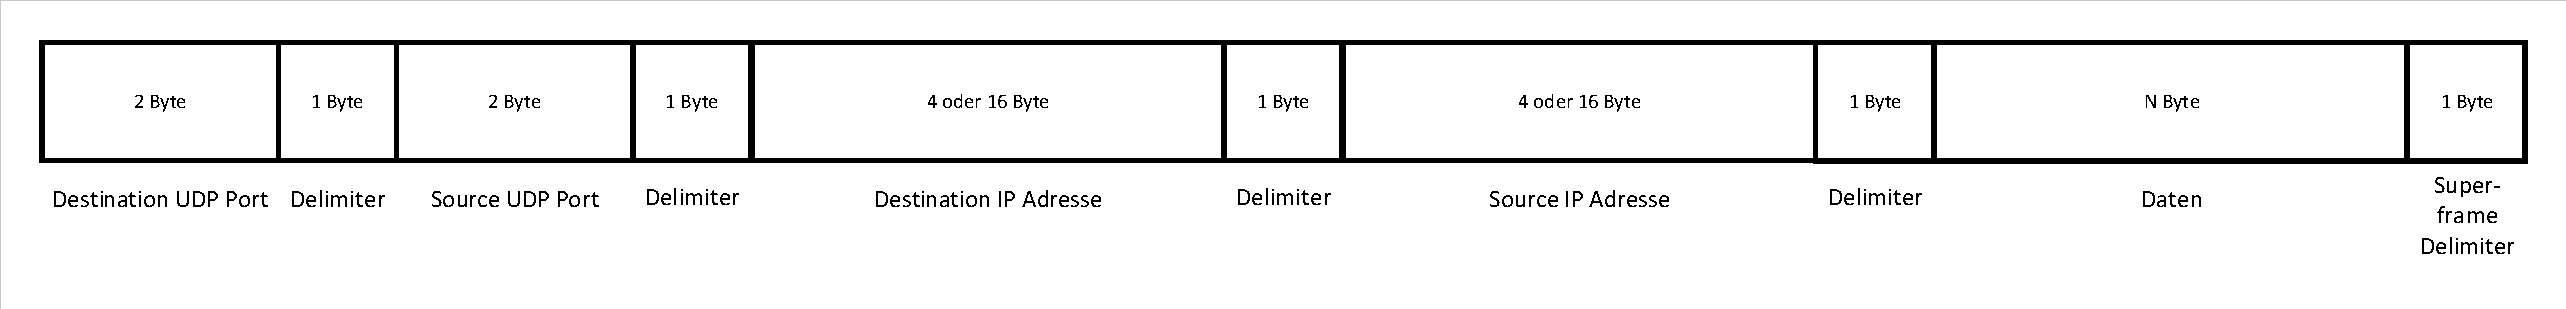
\includegraphics[width=\textwidth]{Grafiken-Alex/komm-extern.pdf}
	\caption{Aufbau eines Routing-Pakets zur UART-Kommunikations. Als Delimiter wird 0x2E (entspricht in ASCII einem Punkt) und als Superframe Delimiter 0x0A (entspricht in ASCII dem New-Line-Character) eingesetzt.}
	\label{komm-intern}
\end{figure}

\subsection{Inbetriebnahme}
Zur Inbetriebnahme muss die Software zunächst kompiliert werden. Zu diesem Zweck bietet sich Instant Contiki an, da es bereits eine funktionierende Toolchain für Contiki mitbringt. Zunächst muss aber die Software noch gemäß den Anforderungen eingestellt werden. Dies geschieht im File configuration.h mit folgenden Defines.
\begin{itemize}
	\item MODE 		
	\item RPLDEVICE	
	\item TARGET		
\end{itemize}
Die Software wurde nicht nur für den tatsächlichen Einsatz, sondern auch zum Debuggen angefertigt. In letzterem Fall werden sämtliche relevante Ereignisse über UART kommentiert. Mit dem Define MODE kann mit den Optionen RELEASE oder DEBUG ausgewählt werden, auf welche Art die Software kompiliert wird. Der Define RPLDEVICE spezifiziert, ob es sich um eine Node oder die Root handelt und kann durch NODE oder ROOT spezifiziert werden. Zu guter Letzt kann bei TARGET für einen bestimmten Prozessor kompiliert werden. Das Target wird zwar auch beim Build Prozess mitgeteilt, aber im Quellcode ändern sich einzelne Kommandos (z.B. der Einsatz des UART Moduls) in Abhängigkeit des verwendeten Targets. Derzeit werden hier die Optionen Z1 (sinnvoll für den Simulator) und CC1310 unterstützt. Beispielsweise könnte die Konfiguration einer Node als Release wie folgt aussehen.\\
\\
\emph{\#define MODE 		RELEASE \\	
	\#define RPLDEVICE	NODE \\	
	\#define TARGET		CC1310 } \\

Zum Kompilieren navigiert man mit der Kommandozeile in den Ordner, an dem das Projekt liegt und gibt den folgenden Build-Command ein: \\
\emph{make TARGET=srf06-cc26xx BOARD=cc1310/launchpad udp-node.bin} \\
Äquivalent dazu lautet der Build-Command für eine Root \\
\emph{make TARGET=srf06-cc26xx BOARD=cc1310/launchpad udp-root.bin} \\
Sollte eine Fehlermeldung, die besagt, dass Contiki nicht gefunden werden konnte, erscheinen, muss im File MAKEFILE in der Zeile \\
\emph{CONTIKI = ../../contiki} \\
der korrekte Pfad zum Ordner von Contiki mitgeteilt werden. Die Standard-Konfiguration funktioniert beispielsweise, wenn der Projektordner auf dem Desktop und Contiki im Home-Folder liegt. Die fertigen Binaries können nun beispielsweise mit dem Flash Programmer 2 geflasht werden. 

\subsection{Übersicht der Befehle zur Steuerung der Teilnehmer}
Für Nodes funktionieren alle Befehle sowohl im DEBUG als auch im RELEASE Modus. Die Root ist im ROOT Modus nicht zur UART-Kommunikation mit Menschen ausgelegt, weshalb hier keine Befehle funktionieren. \\
Da Edge Router und Root die gleiche Firmware benutzen, handelt es sich hier um ein Gerät und beide Begriffe können im Kontext dieses Projekts synonym verwendet werden. \\
\begin{longtable}{l|p{4cm}|p{4cm}|p{2cm}|p{4cm}|p{4cm}}
	\textbf{Kategorie} & \textbf{Befehl} & \textbf{Beschreibung} & \textbf{Gerätetyp} & \textbf{Beispiel} & \textbf{Anmerkung} \\
	\toprule[1.5pt] &&&&&\\
	\textbf{Allgemein} & print id & Zeigt ID von bereitgestelltem Service an. & Node, Root & print id & \\
	\midrule
	& print ip & Zeigt eigene IPv6-Adresse an & Node, Root  & print ip \\
	\midrule
	& hello & Grüßt Teilnehmer und stellt sich vor & Node, Root & hello \\
	& hello device &&&&\\
	\bottomrule[1.5pt] &&&&&\\
	\textbf{Servreg-Hack} & service register [ID] & Stellt Service mit ID [ID] bereit. & Node, Root & service register 150
	& Root registriert im Release automatisch Servive mit ID 190 \\
	\midrule
	& service get ip [ID] & IP von Teilnehmer, der Service mit ID [ID] bereitstellt anzeigen.
	& Node, Root & service get ip 180 \\
	\midrule
	& service edge [ID] & Speichert die ID des Edge Routers. & Node & service edge 190 & Überprüft, ob Root Service mit dieser ID anbietet. \\
	\bottomrule[1.5pt] &&&&&\\
	\textbf{UDP} & udp send id [ID] [DATA] & Sendet Nachricht [DATA] an Teilnehmer mit ID [ID]. & Node, Root & udp send id 190 Hello World! \\
	\midrule
	& udp send ip [IP] [DATA] & Sendet Nachricht [DATA] an Teilnehmer mit IPv6 [IP]. & Node, Root & udp send ip ffd::1 Hello World! & Außer „::“ am Anfang oder Ende und „.“ statt „:“ alle IPv6-Konventionen unterstützt. Es findet keine Überprüfung der eingegebenen IPv6-Adresse statt! \\
	\midrule
	& udp send extern [IP] [PORT] [DATA] & Sendet UDP an Edge-Router, der die Nachricht [DATA] an Teilnehmer mit IPv4 [IP] und Port [PORT] weiterleitet. & Node & udp send extern 192.168.200.99 5005 Hello World! & ID des Edge Routers muss bekannt sein. Zuvor per \emph{service edge [ID]} bereitstellen. \\
	\bottomrule[1.5pt]
	
	
	
	
	
\end{longtable}